% !TeX root = ../thuthesis-example.tex

\chapter{系统实现:大数据机器学习研发管理系统Anylearn}

TBD


\section{概念定义}

TBD


\section{使用场景}

TBD


\section{架构设计}

TBD


\section{功能设计}

TBD


\section{线上环境}

“实践是检验真理的唯一标准”这一理念对于软件尤为重要,敏捷开发方法论中也强调了用户反馈对软件迭代的意义。
为了验证Anylearn的能力并持续打磨其功能性能,2021年7月起,Anylearn在大数据系统软件国家工程研究中心的私有云进行了部署,作为一套公开长活的线上系统对外提供服务,供软件学院、研究中心以及其他相关科研团队使用。

\subsection{集群架构}
Anylearn线上环境中配备了11台高性能GPU服务器,每台服务器配备4张GPU,共计44张,包括24张NVIDIA A100(其中20张为40G显存版,4张为80G显存版)和20张NVIDIA GeForce RTX 3090。
Anylearn依托私有云的网络环境,通过搭建Kubernetes集群池化纳管所有GPU服务器。
Kubernetes集群中使用了私有云的3台虚拟机作为主节点形成控制面,并通过内网负载均衡器与GPU服务器连通,实现了集群的高可用,即任意2个主节点下线均不影响集群任何功能的访问。
集群节点的架构如图\ref{fig:cluster}所示。

\begin{figure}
  \centering
  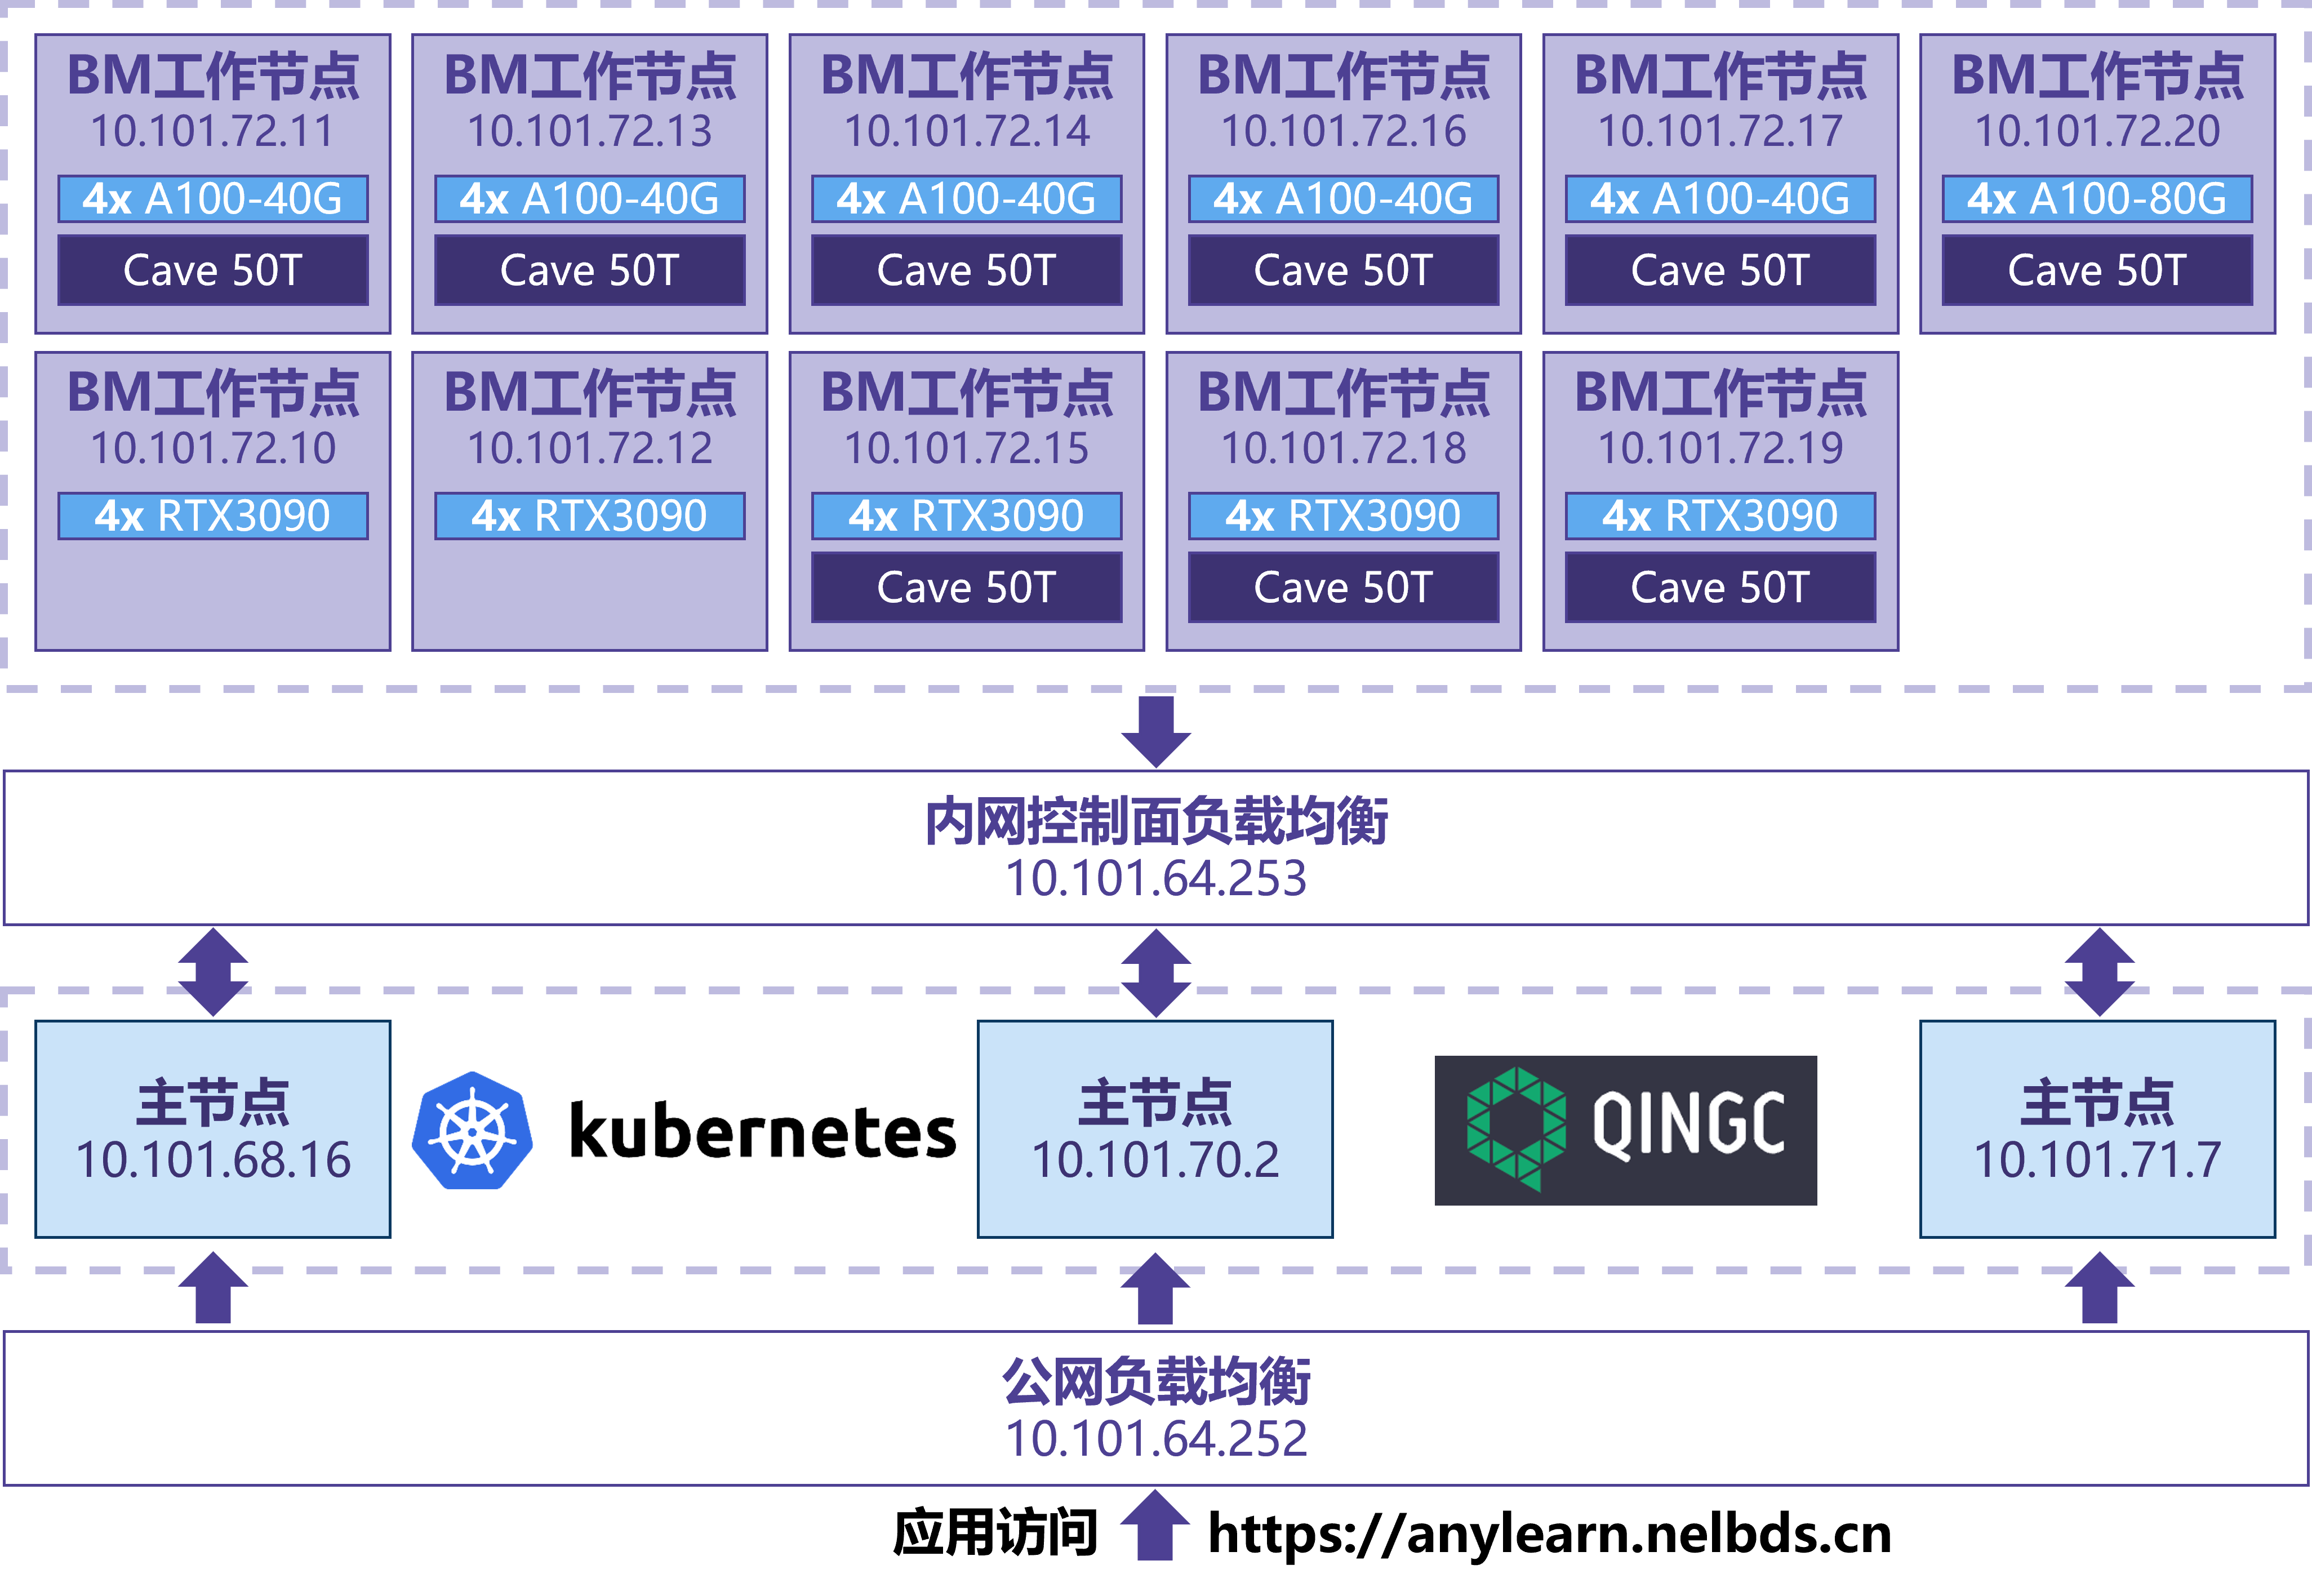
\includegraphics[width=0.8\linewidth]{anylearn-cluster-structure.png}
  \caption{Anylearn线上环境集群架构}
  \label{fig:cluster}
\end{figure}

集群架构经历过7次较大的变动:
(1)2021年7月首次部署时,集群中包含了9台GPU服务器,其中2台未配备GPU,故用作Kubernetes集群控制面的双主节点形成伪高可用架构;
(2)2021年9月,集群中GPU齐备,数量为36张,原用作主节点的2台GPU服务器应当专用于GPU算力负载,不再适合分散其负载能力到控制面,故使用3台私有云虚拟机作为集群主节点,形成真正高可用的集群控制面; 
(3)2022年6月,由于集群证书配置问题导致集群不可用,重新部署了集群并调整了主节点虚拟机的配置;
(4)2022年1月,集群中新增了1台GPU服务器,包含4张NVIDIA GeForce RTX 3090,GPU数量增至40张,扩展操作仅为数条命令,且未影响任何线上业务;
(5)2023年5月,集群中新增了1台GPU服务器,包含4张NVIDIA A100(80G显存版),GPU数量增至44张,扩展操作仅为数条命令,且未影响任何线上业务;
(6)2023年8月,Kubernetes版本从1.21.2逐小版本升级至1.28.1(即1.21.x升级至1.22.x再升级至1.23.x,以此类推直到1.28.1);
(7)2024年3月,由于作为集群主节点的3台私有云虚拟机Linux内核版本过低(4.15),影响了集群网络插件的性能,故重新创建了3台安装了较新版本的Linux内核(5.4)的虚拟机,并将主节点逐一替换,未影响任何线上业务。

\subsection{使用情况}
截至2024年11月14日,Anylearn线上长活环境累计执行了8万8千余次实验,任务执行时长超59万小时,并积累了大量的研发资产,包括近600个共超220TB的数据集、近2万份算法代码和近1600个成品模型。
科研方面,Anylearn支撑了“风清”和“风雷”气象大模型的研发、Timer时序大模型的研发与演示、飞机装配智能调度模型研发与演示等重点项目和重大工程的研究工作,获得了研发人员的高度认可,相关成果发表在《自然》、《中国科学:信息科学》等顶尖期刊。
教学方面,Anylearn支撑了深度学习、大数据基础、软件工程实践等研究生课程和本科生课程,作为模型训练平台为学生提供作业所需的计算资源、训练验证功能、数据集和预训练模型,并为助教和教师提供了作业监管能力。

\begin{table}
  \centering
  \caption{Anylearn线上环境历年使用情况统计}
  \begin{tabular}{crrrrr}
    \toprule
    \multicolumn{1}{c}{年份} & \multicolumn{1}{c}{任务数量} & \multicolumn{1}{c}{执行时长} & \multicolumn{1}{c}{数据集数量} & \multicolumn{1}{c}{算法族数量} & \multicolumn{1}{c}{模型数量} \\
    \midrule
    2021 & 7179 & 26977 & 39 & 619 & 42 \\
    2022 & 27137 & 140655 & 224 & 4715 & 791 \\
    2023 & 35410 & 271001 & 203 & 6336 & 526 \\
    2024 & 18987 & 151588 & 127 & 6993 & 240 \\
    \textbf{总计} & \textbf{88713} & \textbf{590221} & \textbf{593} & \textbf{18663} & \textbf{1599} \\
    \bottomrule
  \end{tabular}
  \label{tab:stats}
\end{table}

表\ref{tab:stats}展示了Anylearn线上环境历年使用情况统计。
其中,2021年系Anylearn集群上线初期,且运行时间仅不到半年,任务数量和执行时长较少。
2022年到2023年是上述科研工作的集中攻关时期,Anylearn整体使用量处于明显的增长态势,尤其体现在任务数量和任务执行时长上,说明Anylearn的功能性能得到了用户的认可,并且在持续完善中。
今年,作为Anylearn线上环境主要用户群的软件学院机器学习组,研究方向逐渐向大规模参数模型发展。
Anylearn集群受限于总体算力和网络带宽,不足以支撑全部的研发工作,因此部分模型训练和验证的任务转向校外算力中心进行,截至11月14日,整体使用量有所下降。


\section{用户案例}

TBD
